\chapter{Dasar Teori}
\label{chap:dasar teori}

Sebelum bisa membuat Twitter bot untuk mencari jalur transportasi publik, berikut diberikan beberapa definisi yang berkaitan dengan pembuatan Twitter bot. Bab ini akan menjelaskan Twitter, Twitter API, KIRI, KIRI API, dan Twitter4j.

\section{Twitter}
\label{sec:twitter}

Twitter adalah layanan yang memungkinkan pengguna untuk mengirim pesan menggunakan 140 karakter atau kurang. Pesan tersebut dapat diadaptasikan melalui teks, aplikasi \textit{mobile}, atau web. (referensi dari buku Sams teach yourself the twitter api) Berikut ini adalah daftar istilah umum pada Twitter:

Twitter adalah salah satu layanan jejaring sosial online yang memungkinkan pengguna memposting pesan berbasis teks hingga 140 karakter (referensi dari buku The Twitter Book).
\begin{itemize}
	\item Tweet 
	
	Posting pada Twitter disebut sebagai \textit{tweet}. \textit{Tweet} ini akan meneruskan pesan singkat yang ditujukan ke semua \textit{follower} suatu akun\footnote{Dusty Reagan, \textit{Twitter Application Development For Dummies}, Wiley, 2010, page 7}. Contohnya adalah seorang akun @kviniink ingin menuliskan bahwa hari ini cuaca cerah, maka @kviniink akan men-tweet 'Hari ini cerah yah..' Tweet juga bisa menyertakan link ke video, foto, atau media lain di internet selain teks biasa. URL link teks termasuk ke dalam 140 batas karakter, namun URL tersebut akan menghabisnya tempat/space dari keterbatasan karakter tweet. Oleh karena itu URL akan dibuat versi singkatnya, contoh saat pengguna memasukkan link 'http://www.chacha.com/gallery/7253/15-movies-that-make-guys-cry', maka akan dibuat menjadi 'bit.ly/1uRi8vV'.
	\item Follow
	
	Follow adalah satu istilah dalam Twitter yang bertujuan untuk mengikuti aktivitas \textit{tweet} suatu akun. Following adalah ketika sebuah akun mengikuti akun orang lain, dan Follower adalah ketika sebuah akun melakukan aksi follow kepada akun anda.
	\item Reply 
	
	Reply adalah cara seseorang untuk dapat memberi rujukan kepada akun Twitter yang lainnya atau lebih dikenal dengan nama \textit{mention}\footnote{Dusty Reagan, \textit{Twitter Application Development For Dummies}, Wiley, 2010, page 9}. Sebagai contoh, diketahui akun bernama @kviniink mem-\textit{follow} @infobdg untuk mengetahui perkembangan apa saja yang tejadi di kota Bandung. Lalu akun @kviniink ingin bertanya tentang info mall yang ramai di Bandung, maka akun @kviniink membuat \textit{mention tweet} yang berisikan "@infobdg Halo saya ingin bertanya apa saja mall yang sedang ramai di Bandung yah?".
	\item Retweet
	
	Retweet ini merupakan salah satu yang paling penting dari Twitter(referensi the twitter book halaman 47). Retweet ini berguna ketika pengguna menemukan tweet menarik dan berbagi tweet tersebut dengan follower akun tersebut (\textit{follower}). Retweet ini juga secara tidak langsung mengatakan bahwa "saya menghormati anda dan pesan yang anda buat".
	
	\item Hashtag
	
	Sebuah fitur yang diciptakan oleh Twitter untuk membantu pencarian kata kunci dan penandaan suatu diskusi.
	
	\item Direct Message(DM)
	
	Direct message digunakan untuk mengirim pesan yang bersifat private antara dua orang. Orang yang mengirim direct message ini hanya bisa untuk orang yang mengikuti akun tersebut.
	\item Timeline
	
	Timeline adalah sekumpulan tweet-tweet dari semua orang yang anda follow lalu akan ditampilkan di halaman utama.
\end{itemize}


	

\section{Twitter API}
Twitter API adalah aplikasi pihak ketiga yang memungkinkan \textit{programmer} melakukan manipulasi dan pengolahan data di Twitter. Twitter API tidak seperti API pada umumnya karena Twitter memaparkan hampir semuanya termasuk setup account dan informasi kustumisasi. Ini adalah salah satu bentuk pendekatan dari Twitter yang berfokus pada jaringan dan memungkinkan developer memiliki hak untuk berpikir 'out of the box' untuk membuat aplikasi yang mereka inginkan. Tetapi tetap akan terjadi keterbatasan yang dimiliki Twitter API, yaitu :
\begin{itemize}
	\item Hanya bisa men-update 1000 per harinya, baik melalui handphone, website, API, dan sebagainya.
	\item Total pesan hanya bisa sebanyak 250 per harinya, pada setiap dan semua perangkat.
	\item 150 permintaan API per jam.
	\item OAuth diijinkan 350 permintaan per jam.
\end{itemize}

Twitter API sendiri dibagi menjadi dua yaitu REST API dan Streaming API.

\subsection{OAuth}
\label{sec:oauth}
Dengan semakin berkembangnya website, semakin banyak situs yang bergantung pada layanan distribusi dan \textit{cloud computing}. Contohnya adalah menggunakan jejaring sosial dengan menggunakan account media sosial lainnya seperti Google untuk mencari teman-teman yang sudah tersimpan pada kontak Google. Atau bisa juga menggunakan pihak ketiga yang memanfaatkan API dari beberapa layanan.

OAuth menyediakan suatu metode bagi pengguna untuk memberi akses pihak ketiga untuk resources (sumber daya) mereka tanpa berbagi password mereka.Cara ini juga memberikan cara untuk memberikan akses yang terbatas(dalam satu lingkup atau durasi) Sebagai contoh, seorang pengguna web dapat memberikan layanan percetakan(client) untuk mengakses foto pribadinya yang disimpan di layanan berbagi foto(server) tanpa harus memberikan username dan passwordnya. Ia akan mengotentikasi langsung dengan layanan berbagi foto tersebut yang mengeluarkan layanan percetakan.

Dalam model otentikasi client-server tradisional, klian menggunakan kredensial untuk mengakses recources hosted oleh server. Di dalam model OAuth, klien (bukan pemilik resource, tetapi bertindak atas namanya) meminta aksesn ke resource yang dikenalkan oleh pemilik resource namun diselenggarakan oleh server.

Agar klien dapat mengakses resource, pertama-tama ia harus mendapatkan izin dari si pemilik resource. Izin ini dinyatakan dalam bentuk token dan mencocokan \textit{shared-secret}. tujuan dari token ini adalah untuk membuat pemilik resource untuk berbagi kepercayaan kepada klien. Berbeda dengan kepercayaan pemilik resource. Token dapat dikeluarkan dalam ruang lingkup terbatas, durasi yang terbatas, dan akan dicabut secara independen. Reverensi(http://hueniverse.com/oauth/guide/intro/)

Twitter OAuth yang diberikan memiliki fitur
\begin{itemize}
	\item secure
	
	Pengguna tidak harus berbagi password mereka dengan aplikasi pihak ketiga untuk meningkatkan keamanan akun.
	\item Standard
	
	Contoh code yang diberikan sudah kompatibel dengan implementasi Twitter OAuth.
\end{itemize}

Twitter sekarang memanfaatkan OAuth 1.0A . Otententikasi aplikasi pengguna adalah bentuk paling umum dari otentikasi resource dalam pelaksanaan OAuth 1.0A Twitter sampai saat ini. Permintaan anda menandatangani baik untuk mengidentifikasi identitas aplikasi anda yang akan menyertakan izin untuk diberikan kepada pengguna. Hal ini bertujuan untuk dapat membuat panggilan API atas nama anda yang diwakili oleh akses token.

\subsubsection{Application-only authentication}
Twitter menawarkan aplikasi yang mampu mengeluarkan permintaan otentifikasi atas nama aplikasi itu sendiri. Dengan menggunakan Application-only authentication  anda tidak mempunyai konteks dari otentikafikasi pengguna dan ini berarti setiap request API untuk endpoint akan membutuhkan konteks user, seperti memposting tweet tidak akan bekerja. Aplikasi yang akan di dapat adalah: 

\begin{itemize}
	\item Melihat timeline
	\item Mengakses following dan follower dari suatu akun
	\item Mencari dalam tweet
	\item mengambil informasi dari akun manapun
\end{itemize}


Tetapi application-only authentication tidak bisa melakukan :

\begin{itemize}
	\item Posting tweet
	\item Melakukan koneksi dengan Streaming endpoint
	\item Mencari akun seseorang
	\item menggunakan geo endpoint manapun
	\item mengakses DM
\end{itemize}

Auth Flow
Langkah-langkah dari application-only auth terdiri dari beberapa langkah yaitu :
Sebuah aplkasi dikodekan berdasarkan \textit{consumer key} dan \textit{secret} ke dalam satu set khusus yang dikodekan secara kredensial.
Aplikasi membuat \textit{request} ke POST OAuth2/token endpoint untuk merubah kredensial tersebut untuk \textit{token bearer}.
Ketika mengakses REST API, aplikasi menggunakan \textit{token bearer} untuk otentifikasi.
Kerena tidak ada kebutuhan duntuk menandatangani request, pendekatan ini lebih sederhana dari model standar OAuth 1.0a

\begin{figure}
	\centering
		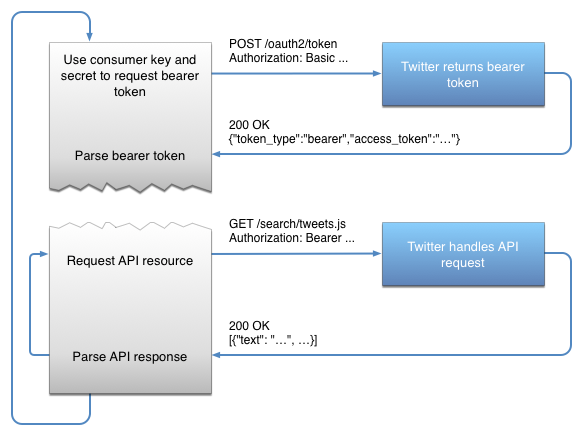
\includegraphics[width=1.00\textwidth]{C:/Users/Kvin/git/Skripsi/doc/DokumenSkripsi/Gambar/flow application-only authentication.png}
	\caption{flow application-only authentication}
	\label{fig:flow application-only authentication}
\end{figure}


Tentang application-only auth
Token adalah \textit{password}. Perlu diingat bahwa \textit{consumer key} dan \textit{secret, bearer token credential}, dan \textit{the bearer token} itu sendiri memberikan akses untuk membuat permintaan atas nama aplikasi itu sendiri. Point-point ini harus dianggap sensitif layaknya password dan tidak boleh dibagikan atau didistribusikan kepada pihak yang tidak dipercaya atau tidak berkepentingan

SSL benar-benar dibutuhkan karena ini adalah cara otentifikasi yang aman. Oleh karena itu semua \textit{request} (baik untuk mendapatkan atau menggunakan token) harus menggunakan endpoint HTTPS, yang juga merupakan syarat untuk menggunakan API v1.1.

Tidak ada konteks pengguna. Ketika mengeluarkan permintaan menggunakan application-only auth, tidak ada konsep \textit{'current-user'}. Karena itu endpoint seperti POST status / update tidak akan berfungsi dengan application-only auth.

\textit{Rate limiting}. \textit{Request} yang dibuat atas nama pengguna tidak akan menguras ketersediaan \textit{rate limit} dan \textit{request} tidak akan menguras batas penggunaan \textbf{limit} dalam \textit{user-based auth}.


\subsubsection{3-legged authorization}
Cara kerja dari 3-legged authorization adalah dengan memberikan aplikasi yang anda buat untuk mengambil \textit{access token} dengan cara melakukan \textit{redirect} user dengan Twitter dan memberikan mereka sebuah otorisasi dari aplikasi yang anda buat. Cara kerja ini hampir identik dengan cara kerja yang dijelaskan pada implementasi \textit{Sign in} dengan Twitter, hanya saja terdapat dua pengecualian yaitu:

\begin{itemize}
	\item \textit{GET oauth endpoint} digunakan sebagai pengganti GET oauth
	\item User akan selalu diminta untuk mengotorisasi akses ke aplikasi anda, bahkan jika akses sebelumnya telah diberikan
\end{itemize}

Beginilah ilustrasi interaksi \textit{sign in} dengan menggunakan \textit{following flowchart}

\begin{figure}[hp]
	\centering
		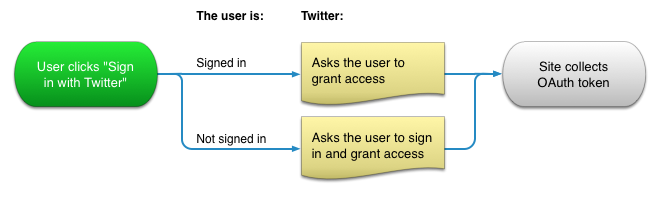
\includegraphics[width=1.00\textwidth]{C:/Users/Kvin/git/Skripsi/doc/DokumenSkripsi/Gambar/sign-in-flow3-3legged.png}
	\caption{Ilustrasi sign in}
	\label{fig:sign-in-flow3-3legged}
\end{figure}

\subsubsection{PIN-based authorization}
cara kerja dari PIN-based authorization ini ditujukan untuk aplikasi yang tidak bisa mengakses atau menanamkan \textit{web browser} untuk mengarahkan user kepada \textit{authorization endpoint}. Contohnya adalah aplikasi yang bersifat \textit{command-line}, \textit{embedded systems}, \textit{game} konsol, dan beberapa jenis aplikasi \textit{mobile}.


Implementasi


Implementasi PIN-based ini memiliki cara kerja yang sama seperti implementasi Sign in dengan Twitter dan \textit{3-legged authorization}, perbedaannya terletak pada nilai dari \textit{oauth$_$callback} yang harus di set menjadi \textit{oob} saat proses pemanggilan \textit{POST oauth/request$_$token}.

Setelah applikasi anda telah mendapatkan \textit{GET oauth/authenticate} atau \textit{GET oauth/authorize URL}, tampilkan URL kepada user agar mereka dapat menggunakan web browser untuk mengakses Twitter.

Ketika \textit{callback oob} diminta dan user pengunjungi Twitter, user tidak akan dipindahkan secara otomatis ke aplikasi setelah menyetujui akses. Sebaliknya, mereka akan melihat PIN code, dengan instruksi untuk kembali ke aplikasi dan memasukkan nilai dari PIN code tersebut.

\begin{figure}[htbp]
	\centering
		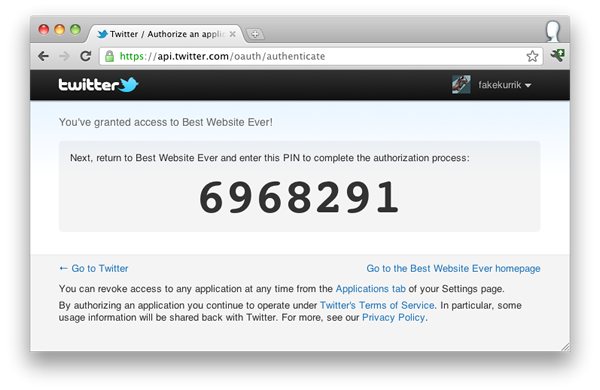
\includegraphics{C:/Users/Kvin/git/Skripsi/doc/DokumenSkripsi/Gambar/pin.png}
	\label{fig:pin}
\end{figure}

Aplikasi anda harus memungkinkan user untuk memasukkan \textit{PIN code} ini untuk menyelesaikan flow tersebut.Nilai dari \textit{PIN code} harus lolos sebagai oauth$_$verifier untuk \textit{POST oauth/access$_$token request}. semua request akan berjalan normal kedepannya.

\subsection{REST API}

REST API menyediakan akses program untuk membaca dan menulis data Twitter. Data tersebut seperti menuliskan tweet baru, membaca profile, melihat follower, dan lainnya. REST API mengidentifikasi aplikasi Twitter dan pengguna menggunakan OAuth.

\subsection{Streamming API}
Streamming API adalah contoh \textit{real-time} API. API ini ditujukan bagi para pengembang dengan kebutuhan data yang intensif. Contohnya jika mencari cara untuk membangun sebuah data produk data-mining atau tertarik dalam analisis penelitian. Streaming API memungkinkan melacak kata kunci yang ditentukan dalam jumlah besar dan melakukan suatu aksi (seperti tweet) secara langsung atau \textit{real-time}.

Twitter menawarkan beberapa endpoint streaming, disesuaikan dengan kasus yang terjadi. 
\begin{itemize}
	\item Public stream
	
	Steaming data publik yang mengalir melalui Twitter. Dipergunakan untuk mengikuti sebuah akun atau topik tertentu. Selain itu juga public stream digunakan untuk data mining.
	\item User Stream
	
	Single-user streams, mengandung hampir semua data korespondensi ...
	
	\item Site Stream
	
	Versi dari multi-user stream. Site stream harus terhubung dengan server yang terkoneksi dengan twitter atas nama banyak pengguna.
\end{itemize}

Perbedaan antara Streaming API dan REST API yaitu ...



%\section{KIRI}
%\label{sec:kiri}
%KIRI adalah sebuah situs atau \textit{website} yang memberi panduan tentang jalur transportasi publik. Alasan KIRI dapat berdiri adalah karenanya global warming, kemacetan, harga bensin yang semakin mahal. Ketiga alasan tersebut yang menjadi masalah sekarang ini, dan semua itu dapat diatasi dengan menaiki transportasi publik. 

%Peran dari KIRI ini adalah memberitahukan seseorang jalur transportasi publik dari satu tempat ke tempat yang dituju. Adapula format yang harus diisi dalam melakukan pencarian ini yaitu
%\begin{enumerate}
%	\item kota,
%	\item tempat awal,
%	\item tempat tujuan.
%\end{enumerate}

\section{KIRI API}
KIRI API adalah aplikasi pihak ketiga yang memungkinkan \textit{programmer} mendapatkan data tentang info jalur transportasi publik. KIRI API dapat diakses dengan beberapa cara. Semua request harus berisikan API key, yang dapat diambil melalui KIRI API Management Dashboard. Berikut adalah spesifikasi dari KIRI API

\begin{itemize}
	\item Routing Web Service
	\item Search Place Web Service
	\item Nearest Transports Web Service
\end{itemize}